 \documentclass{beamer}
\usetheme{tokitex}

\usepackage{tikz}
\usepackage{graphics}
\usepackage{multirow}
\usepackage{tabto}
\usepackage{xspace}
\usepackage{amsmath}
\usepackage{hyperref}
\usepackage{wrapfig}
\usepackage{mathtools}

\usepackage{tikz}
\usepackage{clrscode3e}
\usepackage{gensymb}

\usepackage[english,bahasa]{babel}
\newtranslation[to=bahasa]{Section}{Bagian}
\newtranslation[to=bahasa]{Subsection}{Subbagian}

\usepackage{listings, lstautogobble}
\usepackage{color}

\definecolor{dkgreen}{rgb}{0,0.6,0}
\definecolor{gray}{rgb}{0.5,0.5,0.5}
\definecolor{mauve}{rgb}{0.58,0,0.82}

\lstset{frame=tb,
  language=c++,
  aboveskip=0mm,
  belowskip=0mm,
  showstringspaces=false,
  columns=fullflexible,
  keepspaces=true,
  basicstyle={\small\ttfamily},
  numbers=none,
  numberstyle=\tiny\color{gray},
  keywordstyle=\color{blue},
  commentstyle=\color{dkgreen},
  stringstyle=\color{mauve},
  breaklines=true,
  breakatwhitespace=true,
  lineskip={-3pt}
}

\usepackage{caption}
\captionsetup[figure]{labelformat=empty}

\newcommand{\progTerm}[1]{\textbf{#1}}
\newcommand{\foreignTerm}[1]{\textit{#1}}
\newcommand{\newTerm}[1]{\alert{\textbf{#1}}}
\newcommand{\emp}[1]{\alert{#1}}
\newcommand{\statement}[1]{"#1"}

\newcommand{\floor}[1]{\lfloor #1 \rfloor}
\newcommand{\ceil}[1]{\lceil #1 \rceil}
\newcommand{\abs}[1]{\left\lvert#1\right\rvert}
\newcommand{\norm}[1]{\left\lVert#1\right\rVert}

% Getting tired of writing \foreignTerm all the time
\newcommand{\farray}{\foreignTerm{array}\xspace}
\newcommand{\fArray}{\foreignTerm{Array}\xspace}
\newcommand{\foverhead}{\foreignTerm{overhead}\xspace}
\newcommand{\fOverhead}{\foreignTerm{Overhead}\xspace}
\newcommand{\fsubarray}{\foreignTerm{subarray}\xspace}
\newcommand{\fSubarray}{\foreignTerm{Subarray}\xspace}
\newcommand{\fbasecase}{\foreignTerm{base case}\xspace}
\newcommand{\fBasecase}{\foreignTerm{Base case}\xspace}
\newcommand{\ftopdown}{\foreignTerm{top-down}\xspace}
\newcommand{\fTopdown}{\foreignTerm{Top-down}\xspace}
\newcommand{\fbottomup}{\foreignTerm{bottom-up}\xspace}
\newcommand{\fBottomup}{\foreignTerm{Bottom-up}\xspace}
\newcommand{\fpruning}{\foreignTerm{pruning}\xspace}
\newcommand{\fPruning}{\foreignTerm{Pruning}\xspace}

\newcommand{\fgraph}{\foreignTerm{graph}\xspace}
\newcommand{\fGraph}{\foreignTerm{Graph}\xspace}
\newcommand{\froot}{\foreignTerm{root}\xspace}
\newcommand{\fRoot}{\foreignTerm{Root}\xspace}
\newcommand{\fnode}{\foreignTerm{node}\xspace}
\newcommand{\fNode}{\foreignTerm{Node}\xspace}
\newcommand{\fedge}{\foreignTerm{edge}\xspace}
\newcommand{\fEdge}{\foreignTerm{Edge}\xspace}
\newcommand{\fcycle}{\foreignTerm{cycle}\xspace}
\newcommand{\fCycle}{\foreignTerm{Cycle}\xspace}
\newcommand{\fdegree}{\foreignTerm{degree}\xspace}
\newcommand{\fDegree}{\foreignTerm{Degree}\xspace}
\newcommand{\fadjacencylist}{\foreignTerm{adjacency list}\xspace}
\newcommand{\fAdjacencylist}{\foreignTerm{Adjacency list}\xspace}
\newcommand{\fadjacencymatrix}{\foreignTerm{adjacency matrix}\xspace}
\newcommand{\fAdjacencymatrix}{\foreignTerm{Adjacency matrix}\xspace}
\newcommand{\fedgelist}{\foreignTerm{edge list}\xspace}
\newcommand{\fEdgelist}{\foreignTerm{Edge list}\xspace}
\newcommand{\flist}{\foreignTerm{list}\xspace}
\newcommand{\fList}{\foreignTerm{List}\xspace}
\newcommand{\fgraphtraversal}{\foreignTerm{graph traversal}\xspace}
\newcommand{\fGraphtraversal}{\foreignTerm{Graph traversal}\xspace}
\newcommand{\ftree}{\foreignTerm{tree}\xspace}
\newcommand{\fTree}{\foreignTerm{Tree}\xspace}
\newcommand{\fsubtree}{\foreignTerm{subtree}\xspace}
\newcommand{\fSubtree}{\foreignTerm{Subtree}\xspace}
\newcommand{\fparent}{\foreignTerm{parent}\xspace}
\newcommand{\fParent}{\foreignTerm{Parent}\xspace}
\newcommand{\fsibling}{\foreignTerm{sibling}\xspace}
\newcommand{\fSibling}{\foreignTerm{Sibling}\xspace}
\newcommand{\fpath}{\foreignTerm{path}\xspace}
\newcommand{\fPath}{\foreignTerm{Path}\xspace}
\newcommand{\fconnectedcomponent}{\foreignTerm{connected component}\xspace}
\newcommand{\fConnectedcomponent}{\foreignTerm{Connected component}\xspace}
\newcommand{\fbridge}{\foreignTerm{bridge}\xspace}
\newcommand{\fBridge}{\foreignTerm{Bridge}\xspace}
\newcommand{\farticulationpoint}{\foreignTerm{articulation point}\xspace}
\newcommand{\fArticulationpoint}{\foreignTerm{Articulation point}\xspace}
\newcommand{\ftreeedge}{\foreignTerm{tree edge}\xspace}
\newcommand{\fTreeedge}{\foreignTerm{Tree edge}\xspace}
\newcommand{\fbackedge}{\foreignTerm{back edge}\xspace}
\newcommand{\fBackedge}{\foreignTerm{Back edge}\xspace}
\newcommand{\fforwardedge}{\foreignTerm{forward edge}\xspace}
\newcommand{\fForwardedge}{\foreignTerm{Forward edge}\xspace}
\newcommand{\fcrossedge}{\foreignTerm{cross edge}\xspace}
\newcommand{\fCrossedge}{\foreignTerm{Cross edge}\xspace}
\newcommand{\fdiscoverytime}{\foreignTerm{discovery time}\xspace}
\newcommand{\fDiscoverytime}{\foreignTerm{Discovery time}\xspace}
\newcommand{\flowlink}{\foreignTerm{low link}\xspace}
\newcommand{\fLowlink}{\foreignTerm{Low link}\xspace}
\newcommand{\fstack}{\foreignTerm{stack}\xspace}
\newcommand{\fStack}{\foreignTerm{Stack}\xspace}
\newcommand{\for}{\foreignTerm{or}\xspace}
\newcommand{\fOr}{\foreignTerm{Or}\xspace}
\newcommand{\fand}{\foreignTerm{and}\xspace}
\newcommand{\fAnd}{\foreignTerm{And}\xspace}
\newcommand{\fcentroid}{\foreignTerm{centroid}\xspace}
\newcommand{\fCentroid}{\foreignTerm{Centroid}\xspace}

\newcommand{\fDivideAndConquer}{\foreignTerm{Divide and conquer}\xspace}
\newcommand{\fdivideAndConquer}{\foreignTerm{divide and conquer}\xspace}
\newcommand{\fMergeSort}{\foreignTerm{Merge sort}\xspace}
\newcommand{\fmergeSort}{\foreignTerm{merge sort}\xspace}
\newcommand{\fQuickSort}{\foreignTerm{Quicksort}\xspace}
\newcommand{\fquickSort}{\foreignTerm{quicksort}\xspace}
\newcommand{\fpivot}{\foreignTerm{pivot}\xspace}
\newcommand{\fPivot}{\foreignTerm{Pivot}\xspace}
\newcommand{\fbruteForce}{\foreignTerm{brute force}\xspace}
\newcommand{\fBruteForce}{\foreignTerm{Brute force}\xspace}
\newcommand{\fCompleteSearch}{\foreignTerm{complete search}\xspace}
\newcommand{\fExhaustiveSearch}{\foreignTerm{exhaustive search}\xspace}
\newcommand{\fbinarySearch}{\foreignTerm{binary search}\xspace}
\newcommand{\fBinarySearch}{\foreignTerm{Binary search}\xspace}
\newcommand{\fternarySearch}{\foreignTerm{ternary search}\xspace}
\newcommand{\fTernarySearch}{\foreignTerm{Ternary search}\xspace}
\newcommand{\funimodal}{\foreignTerm{unimodal}\xspace}
\newcommand{\fUnimodal}{\foreignTerm{Unimodal}\xspace}
\newcommand{\fGreedy}{\foreignTerm{Greedy}\xspace}
\newcommand{\fgreedy}{\foreignTerm{greedy}\xspace}
\newcommand{\fgreedyChoice}{\foreignTerm{greedy choice}\xspace}
\newcommand{\fGreedyChoice}{\foreignTerm{Greedy choice}\xspace}

\newcommand{\fdp}{\foreignTerm{dynamic programming}\xspace}
\newcommand{\fDp}{\foreignTerm{Dynamic programming}\xspace}
\newcommand{\fbitmask}{\foreignTerm{bitmask}\xspace}
\newcommand{\fBitmask}{\foreignTerm{Bitmask}\xspace}
\newcommand{\fstate}{\foreignTerm{state}\xspace}
\newcommand{\fState}{\foreignTerm{State}\xspace}
\newcommand{\fsubmask}{\foreignTerm{submask}\xspace}
\newcommand{\fSubmask}{\foreignTerm{Submask}\xspace}

\newcommand{\pheap}{\foreignTerm{heap}\xspace}
\newcommand{\pHeap}{\foreignTerm{Heap}\xspace}
\newcommand{\pBinaryHeap}{\foreignTerm{Binary Heap}\xspace}
\newcommand{\pbinaryHeap}{\foreignTerm{binary heap}\xspace}
\newcommand{\pHeapsort}{\foreignTerm{Heapsort}\xspace}
\newcommand{\pheapsort}{\foreignTerm{heapsort}\xspace}
\newcommand{\pdjs}{\foreignTerm{disjoint set}\xspace}
\newcommand{\pDjs}{\foreignTerm{Disjoint set}\xspace}

\newcommand{\fdotProduct}{\foreignTerm{dot product}\xspace}
\newcommand{\fDotProduct}{\foreignTerm{Dot product}\xspace}
\newcommand{\fcrossProduct}{\foreignTerm{cross product}\xspace}
\newcommand{\fCrossProduct}{\foreignTerm{Cross product}\xspace}
\newcommand{\fconvexHull}{\foreignTerm{convex hull}\xspace}
\newcommand{\fConvexHull}{\foreignTerm{Convex hull}\xspace}
\newcommand{\fgrahamScan}{\foreignTerm{graham scan}\xspace}
\newcommand{\fGrahamScan}{\foreignTerm{Graham scan}\xspace}
\newcommand{\flineSweep}{\foreignTerm{line sweep}\xspace}
\newcommand{\fLineSweep}{\foreignTerm{Line sweep}\xspace}

\newcommand{\fset}{\foreignTerm{set}\xspace}
\newcommand{\fSet}{\foreignTerm{Set}\xspace}
\newcommand{\fprefixSum}{\foreignTerm{prefix sum}\xspace}
\newcommand{\fPrefixSum}{\foreignTerm{Prefix sum}\xspace}
\newcommand{\ffenwickTree}{\foreignTerm{fenwick tree}\xspace}
\newcommand{\fFenwickTree}{\foreignTerm{Fenwick tree}\xspace}
\newcommand{\frangeSumQuery}{\foreignTerm{range sum query}\xspace}
\newcommand{\fRangeSumQuery}{\foreignTerm{Range sum query}\xspace}
\newcommand{\fquery}{\foreignTerm{query}\xspace}
\newcommand{\fQuery}{\foreignTerm{Query}\xspace}
\newcommand{\fsegmentTree}{\foreignTerm{segment tree}\xspace}
\newcommand{\fSegmentTree}{\foreignTerm{Segment tree}\xspace}
\newcommand{\fbinaryTree}{\foreignTerm{binary tree}\xspace}
\newcommand{\fBinaryTree}{\foreignTerm{Binary tree}\xspace}
\newcommand{\flazyPropagation}{\foreignTerm{lazy propagation}\xspace}
\newcommand{\fLazyPropagation}{\foreignTerm{Lazy propagation}\xspace}
\newcommand{\fsparseTable}{\foreignTerm{sparse table}\xspace}
\newcommand{\fSparseTable}{\foreignTerm{Sparse table}\xspace}

\newcommand{\ftrail}{\foreignTerm{trail}\xspace}
\newcommand{\fTrail}{\foreignTerm{Trail}\xspace}
\newcommand{\feulerTour}{\foreignTerm{euler tour}\xspace}
\newcommand{\fEulerTour}{\foreignTerm{Euler tour}\xspace}
\newcommand{\feulerTourTree}{\foreignTerm{euler tour tree}\xspace}
\newcommand{\fEulerTourTree}{\foreignTerm{Euler tour tree}\xspace}

\newcommand{\fmaxflow}{\foreignTerm{maximum flow}\xspace}
\newcommand{\fMaxflow}{\foreignTerm{Maximum flow}\xspace}
\newcommand{\fmincut}{\foreignTerm{minimum cut}\xspace}
\newcommand{\fMincut}{\foreignTerm{Minimum cut}\xspace}
\newcommand{\fflow}{\foreignTerm{flow}\xspace}
\newcommand{\fFlow}{\foreignTerm{Flow}\xspace}
\newcommand{\fsource}{\foreignTerm{source}\xspace}
\newcommand{\fSource}{\foreignTerm{Source}\xspace}
\newcommand{\fsink}{\foreignTerm{sink}\xspace}
\newcommand{\fSink}{\foreignTerm{Sink}\xspace}
\newcommand{\fbackEdge}{\foreignTerm{back-edge}\xspace}
\newcommand{\fBackEdge}{\foreignTerm{Back-edge}\xspace}
\newcommand{\fresidualCapacity}{\foreignTerm{residual capacity}\xspace}
\newcommand{\fResidualCapacity}{\foreignTerm{Residual capacity}\xspace}
\newcommand{\fbottleneck}{\foreignTerm{bottleneck}\xspace}
\newcommand{\fBottleneck}{\foreignTerm{Bottleneck}\xspace}
\newcommand{\faugmentingPath}{\foreignTerm{augmenting path}\xspace}
\newcommand{\fAugmentingPath}{\foreignTerm{Augmenting path}\xspace}


\title{Greedy}
\author{Tim Olimpiade Komputer Indonesia}
\date{}

\begin{document}

\begin{frame}
  \titlepage
\end{frame}

\begin{frame}
  \frametitle{Pendahuluan}
  Melalui dokumen ini, kalian akan:
  \begin{itemize}
    \item Memahami konsep \fgreedy.
    \item Menyelesaikan beberapa contoh persoalan \fgreedy sederhana.
  \end{itemize}
\end{frame}

\begin{frame}
  \frametitle{Greedy}
  \begin{center}
    \newTerm{\fGreedy} merupakan sebuah teknik dalam strategi penyelesaian masalah, bukan suatu algoritma khusus.
  \end{center}
\end{frame}

\begin{frame}
  \frametitle{Konsep Greedy}
  Suatu persoalan dapat diselesaikan dengan teknik \fgreedy jika persoalan tersebut memiliki memiliki sifat berikut:
  \begin{itemize}
    \item Solusi optimal dari persoalan dapat ditentukan dari solusi optimal subpersoalan tersebut.
    \item Pada setiap subpersoalan, ada suatu langkah yang bisa dilakukan yang mana langkah tersebut menghasilkan solusi optimal pada subpersoalan tersebut. Langkah ini disebut juga \newTerm{\fgreedyChoice}.
  \end{itemize}
\end{frame}

\begin{frame}
  \frametitle{Contoh Soal: Activity Selection}
  \begin{itemize}
    \item Diberikan $N$ buah aktivitas.
    \item Aktivitas ke-$i$ dinyatakan dalam $(a_i.start, a_i.end)$.
    \item Artinya, aktivitas ini dimulai pada waktu $a_i.start$ dan berakhir pada waktu $a_i.end$.
    \item Pada setiap satuan waktu, Anda dapat mengikuti paling banyak satu aktivitas.
    \item Anda ingin mengatur jadwal sedemikian sehingga Anda bisa ikut aktivitas sebanyak mungkin.
  \end{itemize}
\end{frame}

\begin{frame}
  \frametitle{Contoh Activity Selection}
  \begin{itemize}
    \item Sebagai contoh, diberikan 4 buah aktivitas: $[ (1, 3) , (2, 6), (5, 7),  (8, 9) ]$. \item Anda dapat hadir di 3 aktivitas berbeda yang tidak saling tindih, yaitu $(1, 3), (5, 7), dan (8, 9)$.
  \end{itemize}

  \begin{figure}
    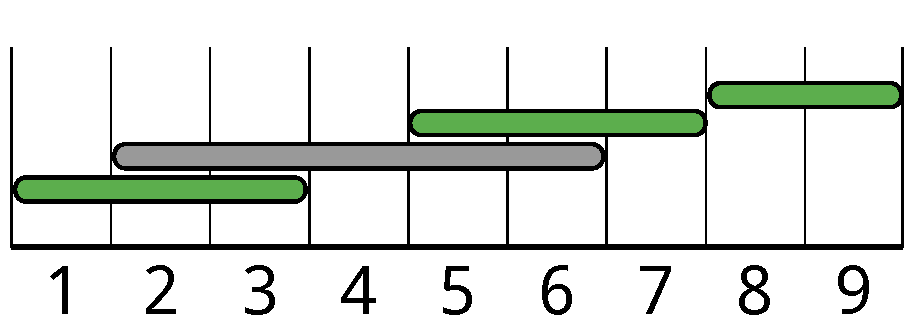
\includegraphics[width=6.5cm]{asset/activity-selection.pdf}
  \end{figure}
\end{frame}

\begin{frame}
  \frametitle{Solusi Activity Selection}
  \begin{itemize}
    \item Misalkan kegiatan pertama yang kita ikuti adalah kegiatan ke-$x$.
    \item Kegiatan selanjutnya yang diikuti haruslah memiliki waktu awal $\geq a_x.end$.
    \item Lebih jauh lagi, ternyata kita mendapat persoalan yang serupa, hanya saja ukurannya lebih kecil.
    \item Dengan kata lain, kita memperoleh subpersoalan.
  \end{itemize}

  \begin{figure}
    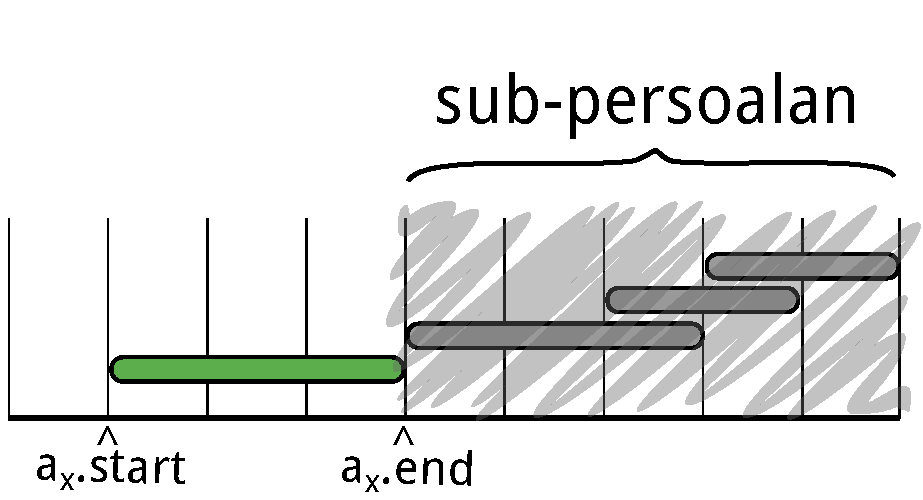
\includegraphics[width=6.5cm]{asset/activity-selection-subproblem.pdf}
  \end{figure}
\end{frame}

%\begin{frame}
%  \frametitle{Solusi Activity Selection (lanj.)}
%  Solusi dari persoalan ini bisa diperoleh dari solusi subpersoalan yang lebih kecil:
%
%  \begin{itemize}
%    \item Kita definisikan $f(t)$ sebagai jumlah aktivitas terbanyak yang dapat diikuti dari waktu ke-1 sampai waktu ke-$t$.
%    \item Jika kita memilih suatu aktivitas $<t' , t>$, maka nilai $f(t) = 1 + f(t' - 1)$
%  \end{itemize}
%\end{frame}
%
%\begin{frame}
%  \frametitle{Solusi Activity Selection (lanj.)}
%  \begin{itemize}
%    \item Artinya, untuk dapat menemukan solusi optimal pada $f(t)$, kita perlu menentukan solusi optimal untuk waktu-waktu yang lebih awal.
%    \item Solusi akhir dari persoalan ini adalah $f(max_e)$, yang mana $max_e$ adalah nilai $a_i.end$ terbesar dari semua pilihan aktivitas yang ada.
%    \item Kita memiliki beberapa pilihan aktivitas yang dapat dipilih, yang mana waktu mulai aktivitas tersebut harus lebih besar dari $t$.
%    \item  \foreignTerm{Greedy choice} untuk permasalah ini adalah dengan memilih aktivitas ke-$k$ yang mana aktivitas tersebut memiliki waktu selesai yang paling cepat.
%    \item Kita bisa hitung solusi dari sub-problem yang lebih besar yaitu $f(a_k.end) = f(t) + 1$. Kita bisa perbarui nilai $t$ menjadi $a_k.end$.
%    \item Jika pada waktu $t$ sudah tidak ada lagi aktivitas yang dapat dipilih, maka nilai $f(t)$ merupakan solusi akhir.
%  \end{itemize}
%\end{frame}

\begin{frame}
  \frametitle{Solusi Activity Selection (lanj.)}
  Pertanyaan: aktivitas mana yg akan pertama kali dipilih?\newline

  Perhatikan pilihan berikut:
  \begin{itemize}
    \item Memilih aktivitas dengan waktu mulai paling awal.
    \item Memilih aktivitas dengan durasi paling singkat.
    \item Memilih aktivitas dengan waktu akhir paling awal.
  \end{itemize}
\end{frame}

\begin{frame}
  \frametitle{Memilih Aktivitas Pertama}
  Memilih aktivitas dengan waktu mulai paling awal:
  \begin{itemize}
    \item Bisa jadi ada aktivitas yang mulai lebih awal, tetapi memiliki durasi yang sangat panjang sehingga menyita waktu.
    \item Memilih aktivitas yang mulai paling awal \emp{belum pasti} optimal.
  \end{itemize}

  \begin{figure}
    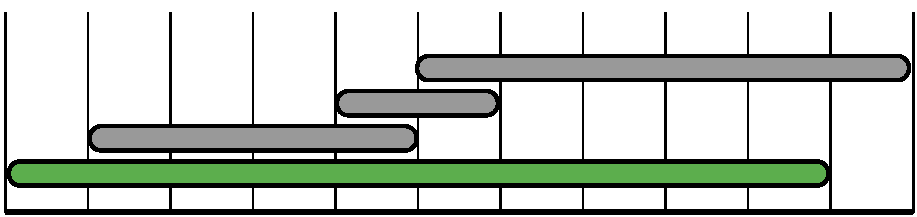
\includegraphics[width=9 cm]{asset/activity-selection-choice-1.pdf}
  \end{figure}
\end{frame}

\begin{frame}
  \frametitle{Memilih Aktivitas Pertama (lanj.)}
  Memilih aktivitas dengan durasi paling singkat:
  \begin{itemize}
    \item Bisa jadi aktivitas dengan durasi paling singkat ini memotong dua aktivitas lain yang sebenarnya dapat kita ikuti.
    \item Pilihan ini juga \emp{belum pasti} menghasilkan solusi optimal.
  \end{itemize}

  \begin{figure}
    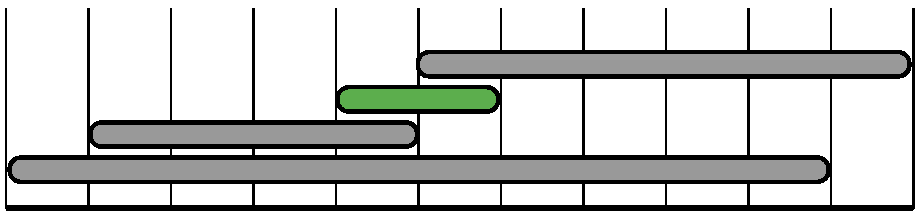
\includegraphics[width=9 cm]{asset/activity-selection-choice-2.pdf}
  \end{figure}
\end{frame}

\begin{frame}
  \frametitle{Memilih Aktivitas Pertama (lanj.)}
  Memilih aktivitas dengan waktu akhir paling awal:
  \begin{itemize}
    \item Dengan memilih aktivitas yang selesai lebih awal, kita mempunyai sisa waktu lebih banyak untuk aktivitas lainnya.
    \item Tanpa peduli kapan aktivitas ini mulai atau berapa durasinya, memilih yang selesai lebih awal \emp{pasti menguntungkan}.
    \item Pilihan ini adalah merupakan \fgreedyChoice, yang \emp{selalu} menghasilkan solusi optimal.
  \end{itemize}

  \begin{figure}
    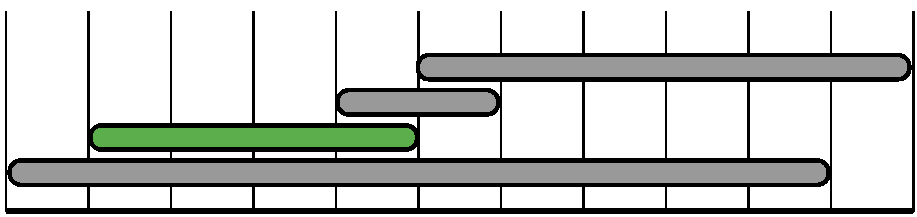
\includegraphics[width=9 cm]{asset/activity-selection-choice-3.pdf}
  \end{figure}
\end{frame}

\begin{frame}
  \frametitle{Penyelesaian Activity Selection}
  \begin{itemize}
    \item Kini kita dapat menentukan aktivitas yang akan diikuti pertama kali.
    \item Selanjutnya kita mendapatkan subpersoalan, yang ternyata dapat diselesaikan dengan cara serupa!
  \end{itemize}
  \begin{figure}
    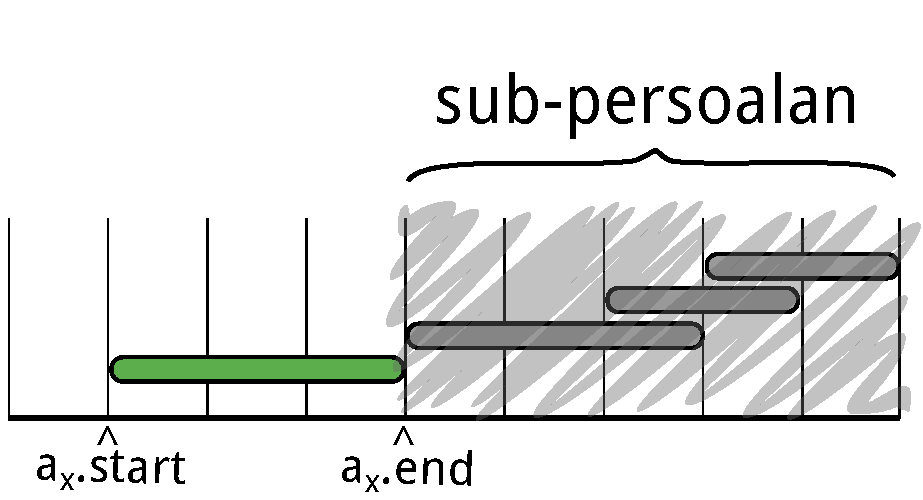
\includegraphics[width=6.5cm]{asset/activity-selection-subproblem.pdf}
  \end{figure}
\end{frame}

\begin{frame}
  \frametitle{Contoh Eksekusi Activity Selection}
  Berikut contoh cara pemilihan aktivitas yang optimal.
  \begin{figure}
    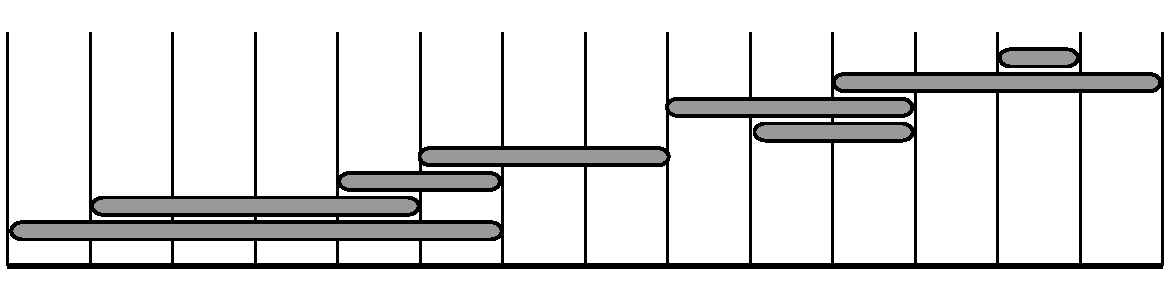
\includegraphics[width=10cm]{asset/activity-selection-algo-1.pdf}
  \end{figure}
\end{frame}

\begin{frame}
  \frametitle{Contoh Eksekusi Activity Selection (lanj.)}
  Dimulai dari memilih aktivitas pertama.
  \begin{figure}
    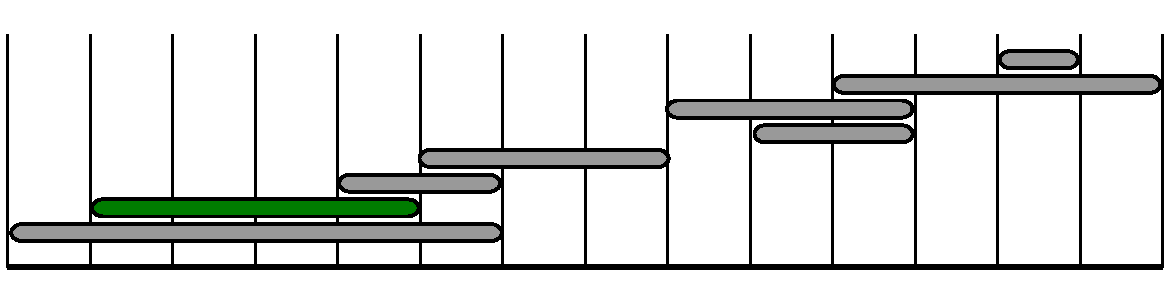
\includegraphics[width=10cm]{asset/activity-selection-algo-2.pdf}
  \end{figure}
\end{frame}

\begin{frame}
  \frametitle{Contoh Eksekusi Activity Selection (lanj.)}
  Selanjutnya kita mendapatkan subpersoalan.

  Beberapa aktivitas kini tidak dapat dipilih lagi.
  \begin{figure}
    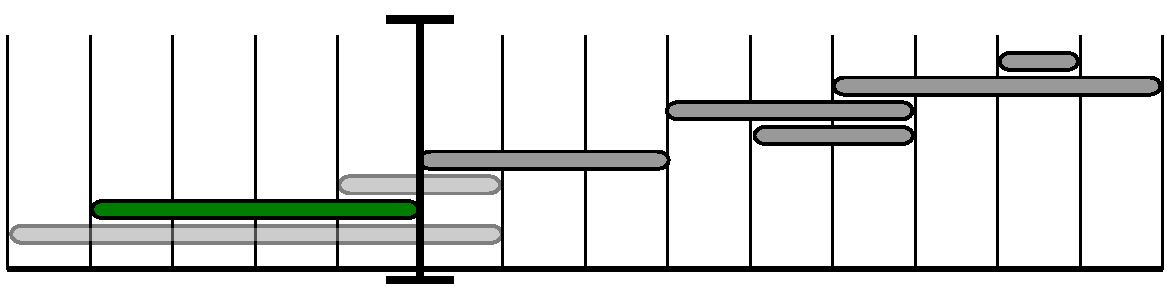
\includegraphics[width=10cm]{asset/activity-selection-algo-3.pdf}
  \end{figure}
\end{frame}

\begin{frame}
  \frametitle{Contoh Eksekusi Activity Selection (lanj.)}
  Masalah yang kita hadapi serupa dengan masalah sebelumnya.

  Kita tinggal memilih aktivitas yang berakhir paling awal.
  \begin{figure}
    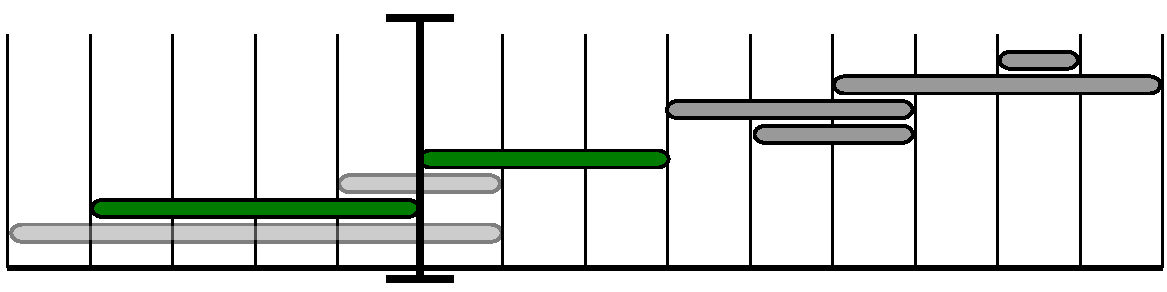
\includegraphics[width=10cm]{asset/activity-selection-algo-4.pdf}
  \end{figure}
\end{frame}

\begin{frame}
  \frametitle{Contoh Eksekusi Activity Selection (lanj.)}
  Kembali kita mendapatkan subpersoalan....
  \begin{figure}
    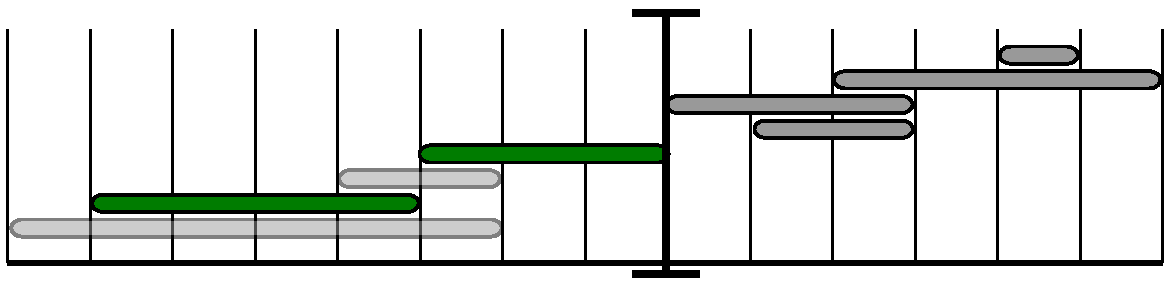
\includegraphics[width=10cm]{asset/activity-selection-algo-5.pdf}
  \end{figure}
\end{frame}

\begin{frame}
  \frametitle{Contoh Eksekusi Activity Selection (lanj.)}
  Pilih lagi aktivitas yang berakhir paling awal.
  \begin{figure}
    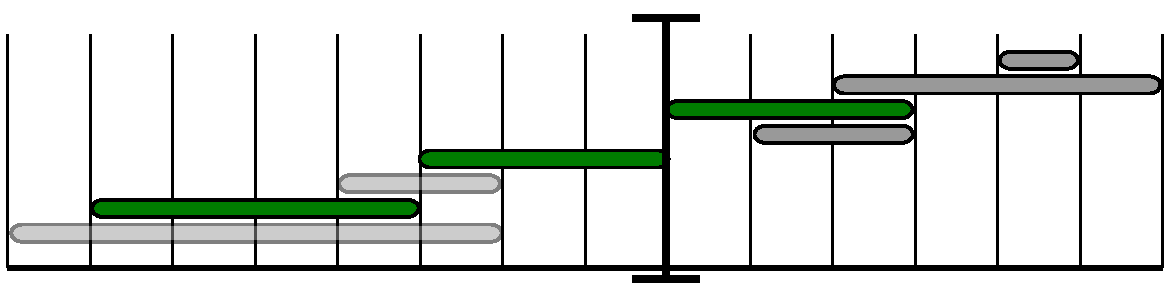
\includegraphics[width=10cm]{asset/activity-selection-algo-6.pdf}
  \end{figure}
\end{frame}

\begin{frame}
  \frametitle{Contoh Eksekusi Activity Selection (lanj.)}
  Didapatkan lagi subpersoalan....
  \begin{figure}
    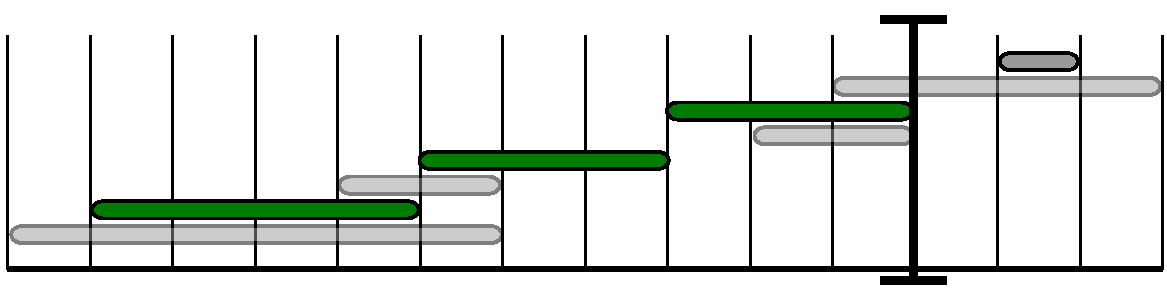
\includegraphics[width=10cm]{asset/activity-selection-algo-7.pdf}
  \end{figure}
\end{frame}

\begin{frame}
  \frametitle{Contoh Eksekusi Activity Selection (lanj.)}
  Pilih lagi aktivitas yang berakhir paling awal.
  \begin{figure}
    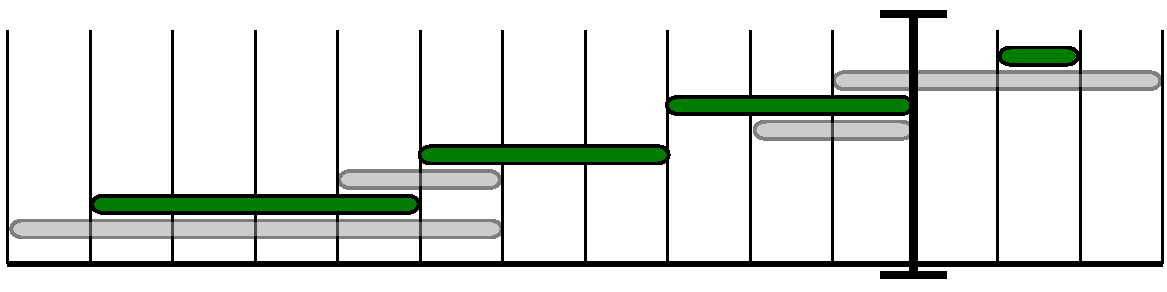
\includegraphics[width=10cm]{asset/activity-selection-algo-8.pdf}
  \end{figure}
\end{frame}

\begin{frame}
  \frametitle{Contoh Eksekusi Activity Selection (lanj.)}
  Selesai!

  Tidak ada cara lain yang memberikan hasil lebih optimal.
  \begin{figure}
    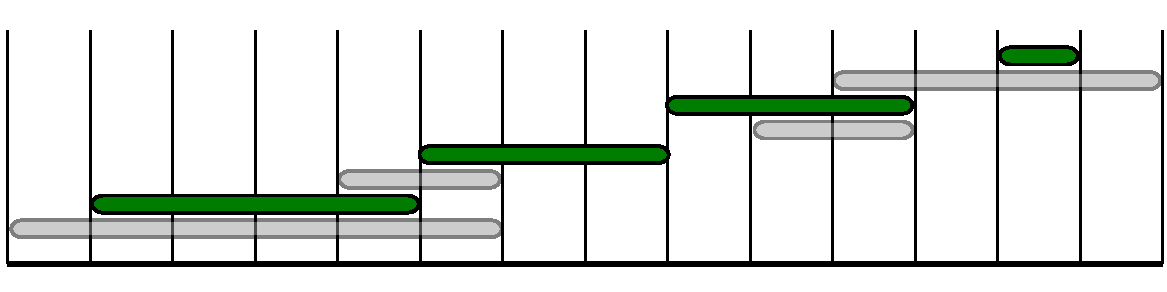
\includegraphics[width=10cm]{asset/activity-selection-algo-9.pdf}
  \end{figure}
\end{frame}

\begin{frame} [fragile]
  \frametitle{Implementasi Solusi Activity Selection}
  \begin{codebox}
    \Procname{$\proc{solveActivitySelection}(a[], N)$}
    \li \Comment Urutkan $a$ secara menaik berdasarkan $a[i].end$
    \li $\proc{sortByEndingTime}(a, N)$
    \zi
    \li $selectedCount \gets 0$
    \li $startTime \gets 1$
    \li \For $i \gets 1$ \To $N$ \Do
    \li   \If $(a[i].start >= startTime)$ \Then
    \li     $selectedCount \gets selectedCount + 1$
    \li     $startTime \gets a[i].end + 1$
          \End
        \End
    \li \Return $selectedCount$
  \end{codebox}
\end{frame}

\begin{frame}
  \frametitle{Analisis Kompleksitas}
  \begin{itemize}
    \item Mengurutkan aktivitas berdasarkan waktu berakhirnya dapat dilakukan dalam $O(N \log{N})$.
    \item Setelah diurutkan, pemilihan aktivitas dapat dilakukan dalam $O(N)$.
    \item Kompleksitas akhirnya $O(N \log{N})$.
    \item Cepat dan efisien!
  \end{itemize}
\end{frame}

\begin{frame}
  \frametitle{Selingan}
  \begin{itemize}
    \item \fGreedyChoice memungkinkan kita untuk memilih suatu keputusan yang dijamin akan menghasilkan solusi optimal, tanpa peduli ke depannya seperti apa.
    \item Hal ini memberi kesan "rakus", yaitu hanya mementingkan masalah yang sedang dihadapi dan selalu mengambil keputusan terbaik saat ini.
    \item Inilah sebabnya teknik ini dinamakan \fgreedy.
  \end{itemize}
\end{frame}

\begin{frame}
  \frametitle{Permasalahan pada Algoritma \fGreedy}
  Perhatikan contoh soal berikut:
  \begin{itemize}
    \item Anda ingin menukar uang Rp12.000 dengan lembaran uang kertas Rp5.000, Rp2.000, dan Rp1.000.
    \item Anda ingin menukar dengan jumlah lembaran sesedikit mungkin.
  \end{itemize}
\end{frame}

\begin{frame}
  \frametitle{Permasalahan pada Algoritma \fGreedy}
  \begin{itemize}
    \item \fGreedyChoice yang terpikirkan adalah dengan memilih lembarandengan nominal terbesar yang mungkin untuk tiap subpersoalan.
    \item Pertama kita pilih lembaran 5000, sehingga tersisa 7000 lagi yang harus dipecah.
    \item Selanjutnya kita pilih 5000 lagi dan menyisakan 2000 untuk dipecah.
    \item Akhirnya, kita pilih 2000 sebagai pecahan terakhir.
    \item Solusi dari kasus ini adalah dengan menggunakan 3 lembaran.
  \end{itemize}
\end{frame}

\begin{frame}
  \frametitle{Permasalahan pada Algoritma \fGreedy (lanj.)}
  \begin{center}
    Dengan soal yang sama, bagaimana jika lembaran rupiah yang beredar bernilai  Rp5.000, \emp{Rp4.000}, dan Rp1.000?
  \end{center}
\end{frame}

\begin{frame}
  \frametitle{Permasalahan pada Algoritma \fGreedy (lanj.)}
  \begin{itemize}
    \item Dengan algoritma \fgreedy, kita akan menukar  12000 dengan lembaran 5000, 5000, 1000, dan 1000.
    \item Padahal ada solusi yang lebih baik, yaitu menggunakan 3 lembaran 4000.
    \item Pada kasus tersebut, \fgreedyChoice yang tidak selalu dapat menghasilkan solusi optimal.
    \item Permasalahan ini tidak dapat diselesaikan oleh algoritma \fgreedy.
    \item (Permasalahan ini bisa diselesaikan dengan algoritma \textit{dynamic programming}, yang akan dibahas pada materi berikutnya.)
  \end{itemize}
\end{frame}

\begin{frame}
  \frametitle{Permasalahan pada Algoritma \fGreedy (lanj.)}
  \begin{itemize}
    \item Pembuktian kebenaran algoritma \fgreedy tidaklah mudah.
    \item Biasanya akan ada beberapa pilihan  \fgreedyChoice yang ada, yang mana tidak semuanya bisa menghasilkan solusi optimal.
    \item Ketika menemukan suatu \fgreedyChoice, sangat dianjurkan untuk menguji kebenaran dari pilihan tersebut sebelum diimplementasikan.
  \end{itemize}
\end{frame}

\begin{frame}
  \frametitle{Permasalahan pada Algoritma \fGreedy (lanj.)}
  \begin{itemize}
    \item Pengujian yang dapat dilakukan adalah dengan mencoba membuat contoh kasus yang dapat menggagalkan \fgreedyChoice tersebut.
    \item Teknik ini biasa disebut \foreignTerm{proof by counterexample}.
    \item Jika ditemukan satu saja contoh kasus yang mana \fgreedyChoice yang diajukan tidak menghasilkan solusi optimal, maka \fgreedyChoice tersebut dinyatakan salah.
    \item Namun, bila Anda tidak bisa menemukan \foreignTerm{counterexample}, \emp{belum tentu} algoritma Anda benar.
  \end{itemize}
\end{frame}

\begin{frame}
\frametitle{Saran}
  \begin{itemize}
    \item Algoritma \fgreedy terkadang mudah untuk dipikirkan dan mudah untuk diimplementasikan, namun sulit untuk dibuktikan kebenarannya.
    \item Pembuktian kebenaran algoritma \fgreedy bisa jadi membutuhkan pembuktian matematis yang kompleks dan memakan waktu.
    \item Pada suasana kompetisi, intuisi dan pengalaman sangat membantu untuk menyelesaikan soal bertipe \fgreedy.
    \item Berhati-hati dan teliti saat mengerjakan soal bertipe \fgreedy. Perhatikan setiap detil yang ada, karena  bisa berakibat fatal.
  \end{itemize}
\end{frame}

\begin{frame}
\frametitle{Penutup}
  \begin{itemize}
    \item Untuk dapat menguasai \fgreedy, Anda perlu banyak berlatih dan berpikir secara cerdik.
    \item Selamat berlatih untuk mengasah "kerakusan" Anda :)
  \end{itemize}
\end{frame}

\end{document}
